\documentclass[crop,tikz]{standalone}% 'crop' is the default for v1.0, before it was 'preview'
%\usetikzlibrary{...}% tikz package already loaded by 'tikz' option
\usetikzlibrary{shapes,snakes}
\begin{document}
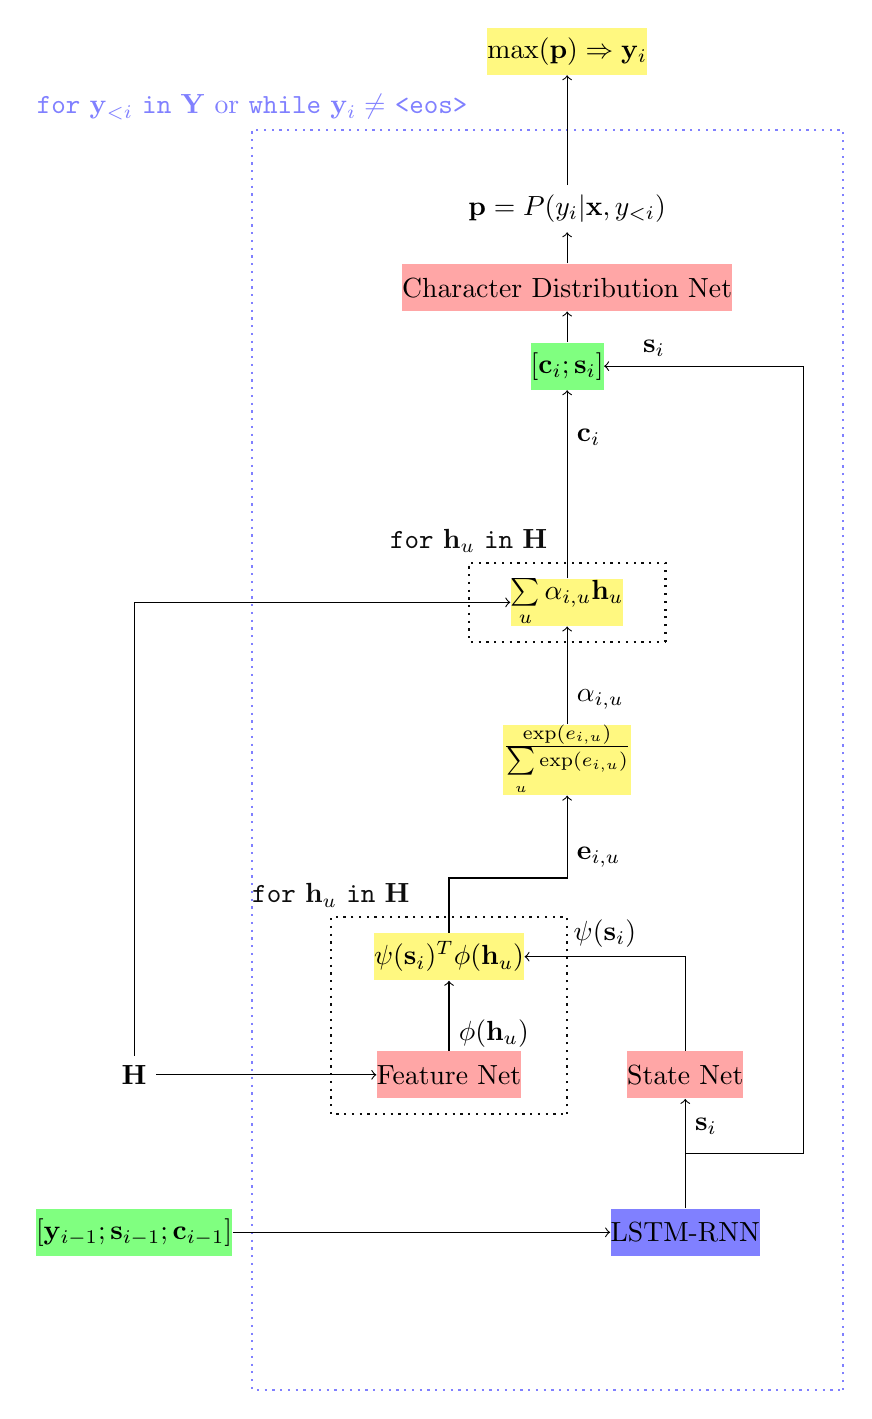
\begin{tikzpicture}
\tikzstyle{operation}=[rectangle,fill=yellow!50,minimum size=17pt,inner sep=0pt]
\tikzstyle{RNN}=[rectangle,fill=blue!50,minimum size=17pt,inner sep=0pt]
\tikzstyle{ffnet}=[rectangle,fill=red!35,minimum size=17pt,inner sep=0pt]
\tikzstyle{merge}=[rectangle,fill=green!50,minimum size=17pt,inner sep=0pt]

%cell box.
\draw[blue!50,thick,dotted] (6,0)  rectangle (-1.5,16) node[above]{\texttt{for} $\mathbf{y}_{<i}$ \texttt{in} $\mathbf{Y}$ or \texttt{while} $\mathbf{y}_i \neq$ \texttt{<eos>}};

\node[merge] (rnn_input) at (-3,2) {$[\mathbf{y}_{i-1}; \mathbf{s}_{i-1};
                                      \mathbf{c}_{i-1}]$};

\node[RNN] (pre_context_rnn) at (4,2) {LSTM-RNN};
\draw[->] (rnn_input) -- (pre_context_rnn);
\node[ffnet] (state_net) at (4,4) {State Net};
\draw[->] (pre_context_rnn) -- (state_net) node[near end, right] {$\mathbf{s}_i$};


\node (high_lvl_features) at (-3,4) {$\mathbf{H}$};
\draw[black!95,thick,dotted] (2.5,3.5)  rectangle (-0.5,6) node[above]{\texttt{for} $\mathbf{h}_u$ \texttt{in} $\mathbf{H}$};
\node[ffnet] (feature_net) at (1,4) {Feature Net};
\draw[->] (high_lvl_features) -- (feature_net);

\node[operation] (scalar_energies) at (1,5.5) {$\psi(\mathbf{s}_i)^T \phi(\mathbf{h}_u)$};
\draw[->] (state_net) |- (scalar_energies) node[near end, above] {$\psi(\mathbf{s}_i)$};
\draw[->] (feature_net) -- (scalar_energies) node[near start, right] {$\phi(\mathbf{h}_u)$};

\node[operation] (softmax) at (2.5,8) {$\frac{\exp(e_{i,u})}{\sum\limits_u \exp(e_{i,u})}$};
\draw[->] (scalar_energies) -- (1,6.5) -- (2.5,6.5) -- (softmax) node[near start, right] {$\mathbf{e}_{i,u}$};

\draw[black!95,thick,dotted] (3.75,9.5)  rectangle (1.25,10.5) node[above]{\texttt{for} $\mathbf{h}_u$ \texttt{in} $\mathbf{H}$ };
\node[operation] (compute_context) at (2.5,10) {$\sum\limits_u \alpha_{i,u} \mathbf{h}_{u}$};
\draw[->] (softmax) -- (compute_context) node[near start, right] {$\alpha_{i,u} $};
\draw[->] (high_lvl_features) |- (compute_context);


\node[merge] (char_dist_net_input) at (2.5,13) {$[\mathbf{c}_i; \mathbf{s}_i]$};
\draw[->] (compute_context) -- (char_dist_net_input) node[near end, right] {$\mathbf{c}_i $};

\node[ffnet] (character_distribution) at (2.5,14) {Character Distribution Net};
\draw[->] (char_dist_net_input) -- (character_distribution);
\draw[->] (pre_context_rnn) -- (4,3) -- (5.5,3) -- (5.5,13) -- (char_dist_net_input) node[near end, above] {$\mathbf{s}_i $};

\node (distribution_value) at (2.5,15) {$\mathbf{p} = P(y_i|\mathbf{x}, y_{<i})$};
\draw[->] (character_distribution) -- (distribution_value);
\node[operation] (one_hot_char) at (2.5,17) {$\max(\mathbf{p}) \Rightarrow \mathbf{y}_i $};
\draw[->] (distribution_value) -- (one_hot_char);


\end{tikzpicture}
\end{document}